\documentclass[12pt]{article}
\usepackage[utf8]{inputenc}
\usepackage[T2A]{fontenc}
\usepackage[russian]{babel}
\usepackage{amsmath,amssymb,graphicx,hyperref}
\usepackage{geometry}
\geometry{a4paper,margin=2.5cm}
\usepackage{bm}
\usepackage{pgf}
\title{Распространение нейтрино высоких энергий через Землю: моделирование и чувствительность к структуре планеты}
\author{В.~А. Аллахвердян, Д.~В. Наумов и С.~И. Завьялов}
\date{\today}

\begin{document}

\maketitle

\begin{abstract}
    Мы представляем подробный анализ прохождения нейтрино сверхвысоких энергий через Землю с учетом взаимодействий по заряженному и нейтральному токам. Используется модель плотности Земли PREM и сечения глубокнонеупругого рассеяния, основанные на партонных распределениях. Мы исследуем область достоверности таких сечений и количественно оцениваем вклад области фазового пространства, в которой отсутствуют измерения. Показано, что при энергиях выше XXX нейтрино начинают чувствительно зондировать ядро Земли, что открывает возможности нейтринной спектроскопии внутренней структуры планеты. Для моделирования сечений разработан пакет \texttt{nudisxs}, а для распространения спектров — \texttt{NuPropagator}, использующий метод $\mathcal{Z}$-фактора. Эти инструменты доступны в открытом виде и могут использоваться для задач нейтринной астрономии и экспериментов типа Baikal-GVD и IceCube.

\end{abstract}

\tableofcontents

\section{Введение}
Современная многоканальная астрономия основывается на объединении данных из различных наблюдательных каналов — электромагнитного излучения (от радиодиапазона до гамма-квантов), гравитационных волн, космических лучей и нейтрино. Такой подход позволяет формировать целостное представление об астрофизических процессах, которое недостижимо при использовании лишь одного вида излучения.

Космические лучи, представляющие собой протоны и атомные ядра, служат инструментом для изучения высокоэнергетических процессов во Вселенной уже более ста лет. Важнейшую роль в этом направлении играют космические лучи сверхвысоких энергий (КЛСВЭ) — частицы с энергией выше $10^9$~ГэВ. Они потенциально связаны с экстремальными астрофизическими объектами и событиями, включая активные ядра галактик, пульсары, сверхновые вспышки~\cite{auger2020anisotropy, auger2020spectrum}, гамма-всплески~\cite{kotera2011astrophysics} и слияния нейтронных звёзд~\cite{kimura2017ultrahigh}. Изучение таких частиц не только углубляет понимание механизмов ускорения до колоссальных энергий, но и открывает возможности для поиска новых физических явлений за пределами Стандартной модели.

Тем не менее, информативность КЛСВЭ ограничивается тремя ключевыми факторами. Во-первых, заряженные частицы отклоняются магнитными полями, что препятствует точной локализации источников. Во-вторых, протоны с энергиями выше $5\times10^{10}$~ГэВ теряют энергию в результате взаимодействия с космическим микроволновым фоном (эффект Грейзена–Зацепина–Кузьмина~\cite{greisen1966}). В-третьих, поток КЛСВЭ чрезвычайно мал по сравнению с потоком нейтрино меньших энергий, что требует детекторов гигантского объёма.

Гамма-астрономия охватывает широкий диапазон энергий фотонов (от 0.1 Мэв до 1 ПэВ), позволяя изучать релятивистские струи, аккреционные диски и пульсары. Современные наземные обсерватории, такие как H.E.S.S.~\cite{hess2021}, MAGIC~\cite{hessandmagic2021}, TAIGA~\cite{Elshoukrofy:2023My} и другие, успешно регистрируют гамма-кванты с энергией до $10^5$~ГэВ. Однако наблюдения в этом диапазоне ограничены межгалактическим поглощением на фоне инфракрасного и микроволнового излучений из-за процессов $\gamma\gamma \to e^+e^-$.

Становление гравитационно-волновой астрономии ознаменовалось регистрацией сигналов от слияний компактных объектов детекторами LIGO и Virgo~\cite{virgoandligo2016}. Эти наблюдения предоставляют уникальные данные о двойных системах и взрывах сверхновых ~\cite{Abbott:2017, Fan:2024}. Преимуществом гравитационных волн является их способность распространяться сквозь вещество без значительных искажений~\cite{Isaacson1968}. Однако эффективность метода ограничивается амплитудой сигнала, которая может оказаться ниже порога чувствительности~\cite{LIGOScientific:2018Sens}.

Особое место среди астрономических инструментов занимают нейтрино сверхвысоких энергий. Благодаря своей нейтральности и крайне слабому взаимодействию с веществом, нейтрино способны достигать детекторов, сохраняя информацию об источнике, даже при прохождении через всю Землю. Эти свойства делают их не только мощным каналом многоканальной астрономии, но и возможным зондом для исследования внутренней структуры планеты.

Важнейшим аспектом интерпретации нейтринных данных является учёт взаимодействия частиц с веществом Земли. С одной стороны, Земля служит поглощающим экраном, ослабляющим нейтринные потоки. С другой — именно это ослабление несёт информацию о плотности вещества и сечениях взаимодействия, открывая возможности для нейтринной томографии.

Современные нейтринные телескопы, такие как IceCube, KM3NeT, Baikal-GVD и другие, располагают эффективными объёмами порядка $0.1$–$1~\text{км}^3$ и регистрируют черенковское излучение, возникающее при взаимодействии нейтрино в прозрачных средах~\cite{Troitskii:2024}. Для моделирования ожидаемых энергетических и угловых спектров требуется точное знание профиля плотности Земли (например, модели PREM), сечений нейтрино-нуклонного взаимодействия в области глубоконеупругого рассеяния, резонансное взаимодействие электронного антинейтрино с электроном, а также учёт процессов регенерации и затухания потока в веществе.

Существующие коллаборации применяют разнообразные подходы к моделированию. В IceCube используются пакеты \texttt{PROPOSAL}~\cite{Koehne:2013gpa} и \texttt{nuSQuIDS}~\cite{ARGUELLES2022108346}, решающие кинетические уравнения с учетом осцилляций нейтрино. KM3NeT реализует собственную  цепочку моделирования, где этапы генерации и распространения разделены~\cite{ARGUELLES2022108346}. 

В рамках настоящей работы разработаны два новых инструмента, предназначенных в первую очередь для моделирования в эксперименте Baikal-GVD, но свободно доступных для всего научного сообщества через платформу \texttt{PyPI}. Пакет \texttt{nudisxs} реализует вычисление дважды дифференциальных сечений глубоконеупругого рассеяния (DIS) с использованием партонных распределений из библиотеки \texttt{LHAPDF6}~\cite{Buckley_2015}. Пакет \texttt{NuPropagator} основан на методе $\mathcal{Z}$-фактора~\cite{Naumov:1998sf} и предназначен для моделирования эволюции нейтринного спектра при прохождении сквозь вещество. Оба инструмента легко интегрируются в существующие симуляционные цепочки и ориентированы на широкое применение в задачах нейтринной астрофизики.

Целями настоящей статьи являются: анализ достоверности глубоконеупругого сечения на ПэВ-ных энергиях с учётом вклада неизмеренного фазового пространства; демонстрация чувствительности нейтринных потоков к структуре земного ядра; описание реализации метода $\mathcal{Z}$-фактора и применение его в задачах моделирования; а также представление и тестирование разработанных инструментов. 
\section{Глубоконеупругое взаимодействие нейтрино с нуклоном}
\subsection{Кинематика и каналы взаимодействия}
Пример глубоконеупругого рассеяния нейтрино  на нуклоне за счет обмена $W$-бозоном, приведен на рис.\ref{fig:DIS}.
\begin{figure}[!h]
\centering
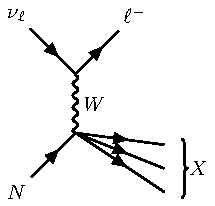
\includegraphics[width=0.4\linewidth]{images/neutrino-nucleon-dis.pdf}
\caption{Диаграмма Фейнмана, соответствующая глубоконеупругому взаимодействию нейтрино с нуклоном через обмен $W$-бозоном.  Существует аналогичная диаграмма с обменом  $Z$-бозоном, при этом $\ell^-\to \nu$.}
\label{fig:DIS}
\end{figure}
Определим кинематические переменные: $k = (E, \bm{k})$ - 4-импульс нейтрино, $k' = (E', \bm{k}')$ 4-импульс  лептона в  конечном состоянии, $p=(M,\bm{0})$ - 4-импульс нуклона, $p'$ - 4-импульс  адронной системы, $q = k-k' = p'-p$. 
Для описания глубоконеупругого события удобно использовать три независимые кинематические переменные: \( Q^2 \), \( x \), \( y \).
Начнём с определения $Q^2$:
\begin{equation}
  Q^2 \equiv -q^2 \approx 2 (EE' - \bm{k} \cdot \bm{k}') \approx 4EE' \sin^2\frac{\theta}{2}.
\end{equation}
Здесь \( \theta \) — угол рассеяния лептона в лабораторной системе. В глубоконеупругом рассеянии \( Q^2 > 0 \).

Переменные Бьёркена:
\begin{equation}
  x = \frac{Q^2}{2(p \cdot q)}, \qquad y = \frac{p \cdot q}{p \cdot k}.
\end{equation}
Кроме того, используются: 
\begin{enumerate}
\item $W^2 = (q+p)^2 = M^2+2 (p\cdot q) -Q^2$ - инвариантный квадрат массы адронов,
\item $s = (k+p)^2$ - квадрат энергии в системе центра масс.
\end{enumerate}

% \subsubsection{Партонная модель}
% Чтобы попытаться написать сечение неупругого взаимодействия, нам нужны распределения партонов в самом нуклоне. Обычно их обозначают f(x), подразумевая, что они носят смысл плотности вероятности числа кварков аромата f, имеющих долю импульса в интервале от $x$ до $x+dx$. Тогда $xf(x)$-плотность вероятности доли
% импульса нуклона, переносимая партонами аромата $f$ с долей импульса в интервале от x до $x+dx$. Из изотопической симметрии следуют следующие очевидные равенства:
% \begin{equation}
% \begin{aligned}
%     f_u^p(x) = f_d^n(x) = u(x), &f_d^p(x) = f_u^n(x) = d(x),&f_s^p(x) = f_s^n(x) = s(x) \\
%     f_{\bar{u}}^p(x) = f_{\bar{d}}^n(x) = \bar{u}(x), &f_{\bar{d}}^p(x) = f_{\bar{u}}^n(x) = \bar{d}(x),&f_{\bar{s}}^p(x) = f_{\bar{s}}^n(x) = \bar{s}(x) \\
% \end{aligned}
% \end{equation}
% На рис.(\ref{DIS1}) можно видеть распределения $xf(x)$ взятых из \cite{ParticleDataGroup:2024cfk}.
% \begin{figure}[!h]
% \includegraphics[width=\linewidth]{"images/NuProp/d3"}
% \caption{Плотность вероятности доли
% импульса нуклона, переносимая партонами \cite{ParticleDataGroup:2024cfk}.}
% \label{DIS1}
% \end{figure}
% Cтандартная классификация, связанная с взаимодействием в электрослабой теории, даётся различием между двумя токами:
% \begin{enumerate}
%     \item Если нейтрино взаимодействует с кварком внутри нуклона через $W^{\pm}$-бозон, то продуктами распада будут является лептоны заряженные лептоны и адроны. Такая мода называется заряженым током (СС-ток).
%     \item Если нейтрино взаимодействует с кварком внутри нуклона через $Z$-бозон, то продуктами распада будут является нейтрино и адроны. Такая мода называется нейтральным током (NС-ток).
% \end{enumerate}

%\subsection{Глубоконеупругое рассеяние}

%Дифференциальное сечение глубоко неупругого рассеяния можно записать в виде:
%\begin{equation}
%    \frac{d^2\sigma}{dxdy} = \frac{2\pi y\alpha^2}{Q^4}\sum\limits_j\eta_jL^{\mu\nu}_jH_{\mu\nu}^j,
%\end{equation}
%где сумма берётся по всем возможным промежуточным бозонам, $eta_j$ - множители, зависящие от промежуточного бозона (например, для фотона он равен 1), а лептонный и адронный тензоры даются выражениями:
%\begin{equation}
%\centering
%\begin{aligned}
%    L_{\mu\nu}(k,k') = &2(k_{\mu}k_{\nu}' + k_{\nu}k_{\mu}' - (kk')g_{\mu\nu} - i\epsilon_{\mu\nu\alpha\beta}k^{\alpha}k'^{\beta})\\
%    H_{\mu\nu}(q,P) = &(-g_{\mu\nu} + \frac{q_{\mu}q_{\nu}}{q^2})F_1(x,Q^2) + \frac{P_{\mu}P_{\nu}}{q^2}F_2(x,Q^2)\\
%    &- i\epsilon_{\mu\nu\alpha\beta}\frac{q^{\alpha}P^{\beta}}{2Pq}F_3(x,Q^2),
%\end{aligned}
%\end{equation}
%где $F_i(x,Q^2)$ — это функции, содержащие информацию о структуре неполяризованного адрона. В итоге, переписывая сечения через структурные функции, можно записать выражения для заряженного и нейтрального тока. 
%\begin{equation}
%\centering
%\begin{aligned}
%    \frac{d^2\sigma}{dxdy} = \frac{2\pi y\alpha^2}{Q^4}\eta_i\left((1-y-x^2y^2M^2/Q^2)F_2^i + y^2xF_1^i ± y(1 - 0.5y)xF_3^i\right)
%\end{aligned}
%\end{equation}
%где $i=NC,CC$, а минус и плюс соответствуют нейтрино и антинейтрино в начальном состоянии соответственно.

\subsection{Общий вид сечения}
Сечения нейтрино-нуклонного глубоконеупругого рассеяния вычисляются по следующей универсальной формуле:
\begin{equation}
    \frac{d^2 \sigma^{\text{DIS}}}{dx\,dy} = \frac{G_F^2 M E}{\pi(1 + Q^2/M_W^2)^2} \sum\limits_{i=1}^{5} A_i(x, y, E)\,F_i(x, Q^2),
    \label{eq:xsec_general}
\end{equation}
где $G_F$ — константа Ферми, $M$ — масса нуклона, $E$ — энергия нейтрино, $Q^2$ — переданный импульс, $F_i(x, Q^2)$ — структурные функции, а $A_i(x, y, E)$ — известные кинематические коэффициенты, зависящие от энергии и переменных Бьёркена $x$ и $y$. 

Структурные функции вычисляются на основе партонных распределений, предоставляемых пользователем. Форма коэффициентов $A_i$ зависит от свойств начальных частиц, в частности, от их поляризации. Подробное описание приведено в приложении~\ref{app:structure_functions}.
\section{Взаимодействие нейтрино с электроном}
Так как сечение взаимодействия нейтрино с электроном много меньше нуклонов, то в дальнейшем будет учитываться только резонанс Глешоу ($\bar{\nu}_e+e^{-}\to W^{+}$). Для расчета будем использовать следующие формулы для дифференциальных сечений, взятые из работы~\cite{GANDHI199681}:
\begin{equation}
    \begin{aligned}
\frac{d\sigma(\bar{\nu}_e e \rightarrow \bar{\nu}_e e)}{dy} 
&= \frac{G_F^2 m E_\nu}{2\pi} \left[ \frac{R_e^2}{\left( 1 + 2m E_\nu y / M_Z^2 \right)^2}\right]\\ 
&+ \frac{G_F^2 m E_\nu}{2\pi}\left[\left| \frac{L_e}{1 + 2m E_\nu y / M_Z^2} + \frac{2}{1 - 2m E_\nu / M_W^2 + i F_w / M_w} \right|^2 (1 - y)^2 \right],\\
\frac{d\sigma(\bar{\nu}_e e \rightarrow \bar{\nu}_\mu \mu)}{dy} 
&= \frac{G_F^2 m E_\nu}{2\pi} \frac{4(1-y)^2 [1-(\mu^2-m^2)/2mE_\nu]^2}{(1-2mE_\nu/M_W^2)^2 + \Gamma_W^2/M_W^2}, \\
\frac{d\sigma(\bar{\nu}_e e \rightarrow \text{hadrons})}{dy} 
&= \frac{d\sigma(\bar{\nu}_e e \rightarrow \bar{\nu}_\mu \mu)}{dy} \frac{\Gamma(W \rightarrow \text{hadrons})}{\Gamma(W \rightarrow \mu \bar{\nu}_\mu)},
\end{aligned}
\end{equation}

\subsection{Программный пакет \texttt{nudisxs}}

\texttt{nudisxs}~\cite{nudisxs2022} — программный модуль на языке Python~3, предназначенный для вычисления сечений нейтрино–нуклонного взаимодействия в области глубоконеупругого рассеяния по формуле~\eqref{eq:xsec_general}. 
Его вычислительное ядро основано на пакете \texttt{XsDis}, написанном на языке Fortran В.~А.~Наумовым и К.~С.~Кузьминым (см., например,~\cite{nudisxs2022}). 
В отличие от исходной версии, рассчитанной на фиксированный набор партонных функций, \texttt{nudisxs} поддерживает динамическую загрузку партонных распределений из библиотеки \texttt{LHAPDF6}~\cite{aartsenLHAPDF2020}.

Модуль позволяет вычислять дважды дифференциальные сечения по переменным Бьёркена~$x$ и~$y$, дифференциальные сечения по одной переменной и полные сечения взаимодействия в широком диапазоне энергий — от сотен~МэВ до~$10^{15}$~ГэВ. 
Он предназначен для задач нейтринной астрофизики и моделирования событий в нейтринных телескопах и может быть легко интегрирован в существующие исследовательские проекты.

Реализация использует библиотеки \texttt{NumPy}~\cite{2020NumPy-Array}, \texttt{SciPy}~\cite{2020SciPy-NMeth} и \texttt{vegas}~\cite{lepageVegas2021} для многомерного Монте–Карло интегрирования, что обеспечивает высокую производительность и удобство при численном анализе и тестировании. 
%

Логическая архитектура пакета \texttt{nudisxs} показана на рис.~\ref{fig:nudisxs1}. 
Основой расчётов является загрузка партонных функций из библиотеки \texttt{LHAPDF6}, используемых для построения структурных функций $F_i(x, Q^2)$, входящих в выражение~\eqref{eq:xsec_general}. 
Пользовательский интерфейс реализован в модуле \texttt{dis}, где задаются тип лептона (нейтрино или антинейтрино), мишень (протон, нейтрон или изоскаляр), энергия нейтрино, минимальное значение $Q^2$, а также выбранный набор партонных распределений и параметров модели. 
Вычисление дважды дифференциальных сечений для заряженного и нейтрального токов выполняют модули \texttt{xs\_cc} и \texttt{xs\_nc}. 
Часть исходного кода, написанного на~Fortran, доступна через интерфейс \texttt{f2py} и обеспечивает быстрые, проверенные временем вычисления ключевых выражений. 
Интерполяция партонных распределений, построение структурных функций и численные процедуры реализованы средствами \texttt{SciPy}.

\begin{figure}[!h]
\centering
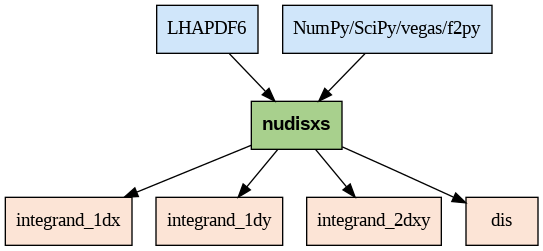
\includegraphics[width=\linewidth]{images/nudisxs_diagram.png}
\caption{Структура программного пакета \texttt{nudisxs} и его зависимости.}
\label{fig:nudisxs1}
\end{figure}

Пакет \texttt{nudisxs} распространяется через платформу \texttt{PyPI} как открытое программное обеспечение. 
Он легко устанавливается и интегрируется в существующие симуляционные цепочки. 
В рамках настоящей работы \texttt{nudisxs} использован для расчёта всех сечений, показанных на рис.~\ref{fig:xsec_2d}–\ref{fig:xsec_total}.

\subsection{Некоторые примеры}

На рис.~\ref{fig:xsec_2d} представлены дважды дифференциальные сечения $\frac{d^2\sigma}{dx\,dy}$ для взаимодействия мюонного нейтрино с протоном через обмен бозоном $W$, рассчитанные при различных энергиях нейтрино и фиксированных значениях переменной $y$. Характерной особенностью этих графиков является то, что с ростом энергии основная часть сечения смещается в область всё меньших значений переменной Бьёркена $x$. Это отражает фундаментальную особенность глубоко-неупругого рассеяния: при больших $Q^2$ всё больший вклад в сечение начинают вносить морские кварки и антикварки.

\begin{figure}[!h]
\centering
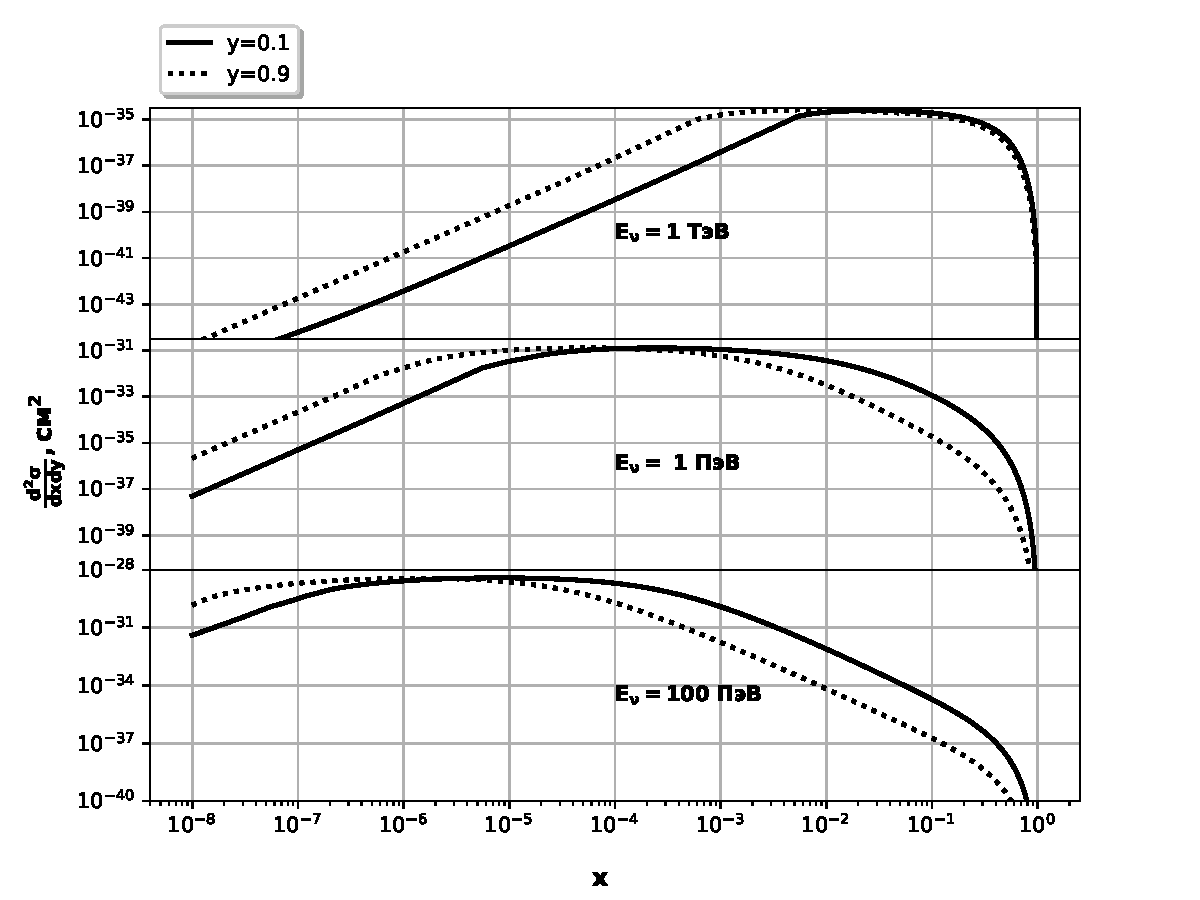
\includegraphics[width=\linewidth]{'images/NuProp/xs_vs_xCT18ZNNLO_cc_12_proton.pdf'}
\caption{Дважды дифференциальные сечения для рассеяния мюонного нейтрино на протоне за счёт заряженного тока в зависимости от переменной Бьёркена $x$ при различных энергиях нейтрино и фиксированных значениях переменной $y$.}
\label{fig:xsec_2d}
\end{figure}

На достаточно высоких энергиях нейтрино (\~ 0.1 ГэВ) достигается область $x \lesssim 10^{-5}$ и ниже, где партонные распределения плохо определены, поскольку соответствующие данные либо отсутствуют, либо экстраполированы из области $x \gtrsim 10^{-4}$. Это приводит к увеличению неопределённости в расчёте полного сечения, особенно при использовании различных наборов PDF.

Оценка вклада неизмеренного фазового пространства в общее сечение — одна из ключевых целей настоящей работы. На рис.~\ref{fig:xsec_total} показана зависимость полного сечения взаимодействия мюонного нейтрино на нуклоне от энергии для различных партонных распределений. Видно, что при $E_\nu \gtrsim 10^5$~ГэВ расчёты, основанные на разных PDF-наборах, начинают расходиться, отражая растущую модельную неопределённость в области малых $x$. Именно в этой области наш подход позволяет количественно оценить вклад недостоверно измеренных компонент, таких как морские кварки и глюоны, в предсказания полного сечения.


\begin{figure}[!h]
\centering
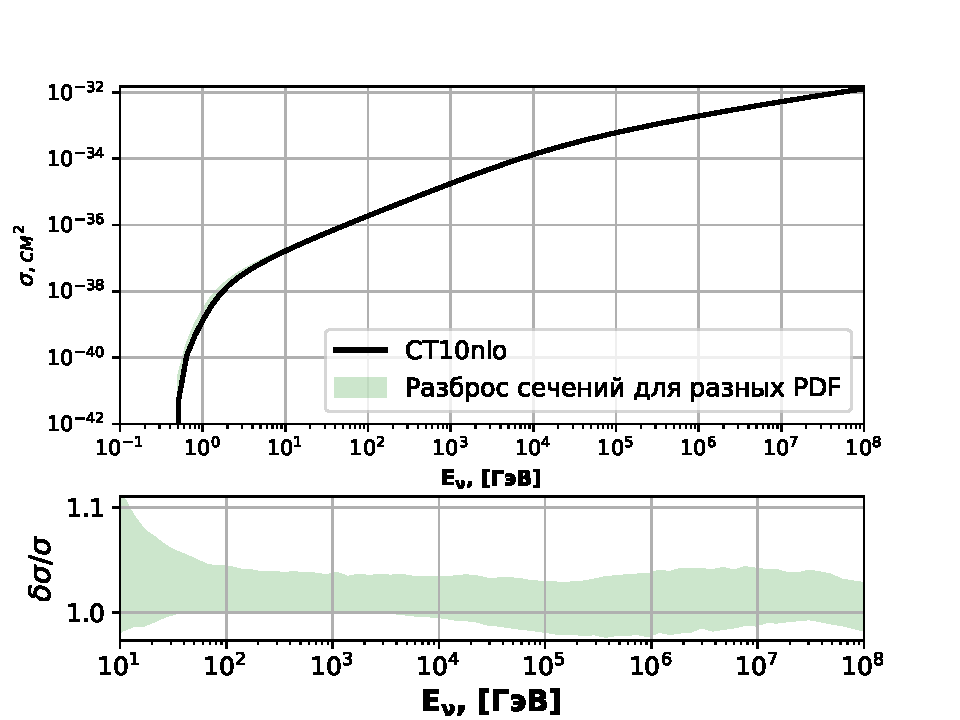
\includegraphics[width=\linewidth]{'images/NuProp/xs_vs_enu.pdf'}
\caption{Полные сечения взаимодействия мюонного нейтрино на нуклоне в зависимости от энергии $E_\nu$ для различных наборов партонных распределений (\texttt{CT18ZNNLO}, \texttt{nCTEQ15}, \texttt{CT10nlo}, \texttt{TUJU19_nlo}). Расхождение при высоких энергиях отражает неопределённость поведения PDF при малых $x$.} 
\label{fig:xsec_total}
\end{figure}

\section{Достоверность партонной модели при ПэВ-энергиях}
\label{sec:dis_reliability}
На рис. (\ref{fig:xQ2_PDG}) приведена исследованная область в экспериментах на коллайдерах:   БАК (LHC), Теватрон, HERA, а также в экспериментах с неподвижной мишенью. В области малых $x\lesssim 10^{-6}$ экспериментальные измерения практически отсутствуют. Между тем, с ростом энергии взаимодействия нейтрино, вклад именно малых $x$ в сечение взаимодействия становится доминирующим. Выход в неисследованную область с необходимостью требует использования экстраполяции, что является источником дополнительной систематической неопределённости. 
\begin{figure}[!h]
\centering
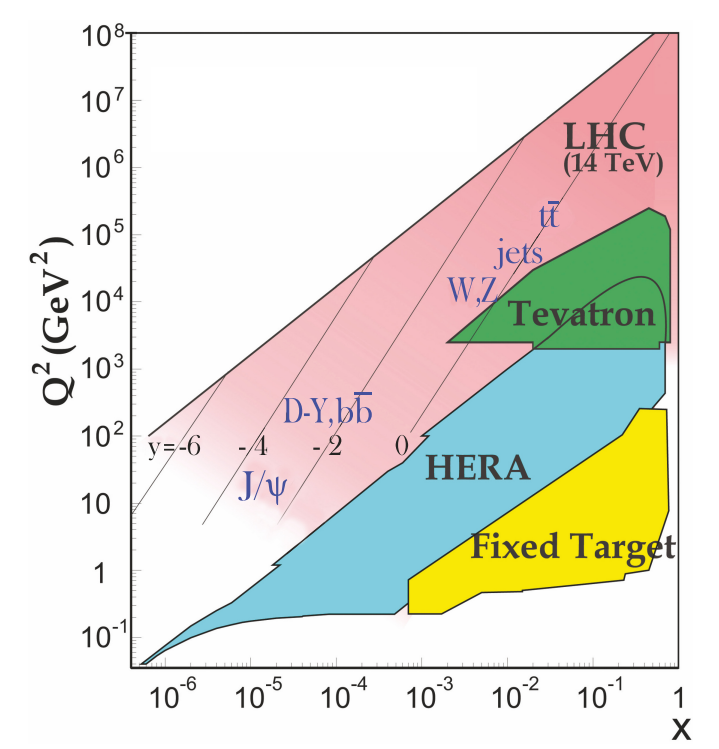
\includegraphics[width=0.8\linewidth]{images/NuProp/reald}
\caption{Кинематические области в $x$ и $Q^2$, исследованные в экспериментах с неподвижной мишенью и на коллайдерах. Рисунок из \cite{ParticleDataGroup:2024cfk}.}
\label{fig:xQ2_PDG}
\end{figure}

\subsection{Вклад экспериментально недоступной области}
Для иллюстрации, на рис.~\ref{fig:diff_xsec_100PeV} приведено дважды дифференциальное нормированное сечение
\[
\frac{1}{\sigma(E_\nu)}\frac{d^2\sigma(E_\nu,x,Q^2)}{dx\,dQ^2}
\] 
как функция переменных $x$ и $Q^2$ при энергии нейтрино $E_{\nu} = 100$ ПэВ. $\sigma(E_\nu)$ - полное сечение глубоконеупругого взаимодействия нейтрино с нуклоном при фиксированной энергии нейтрино. 

На рисунке также приведена заштрихованная область, качественно отражающая экспериментально исследованную область, представленную на рис.~\ref{fig:xQ2_PDG}.
\begin{figure}[!h]
\centering
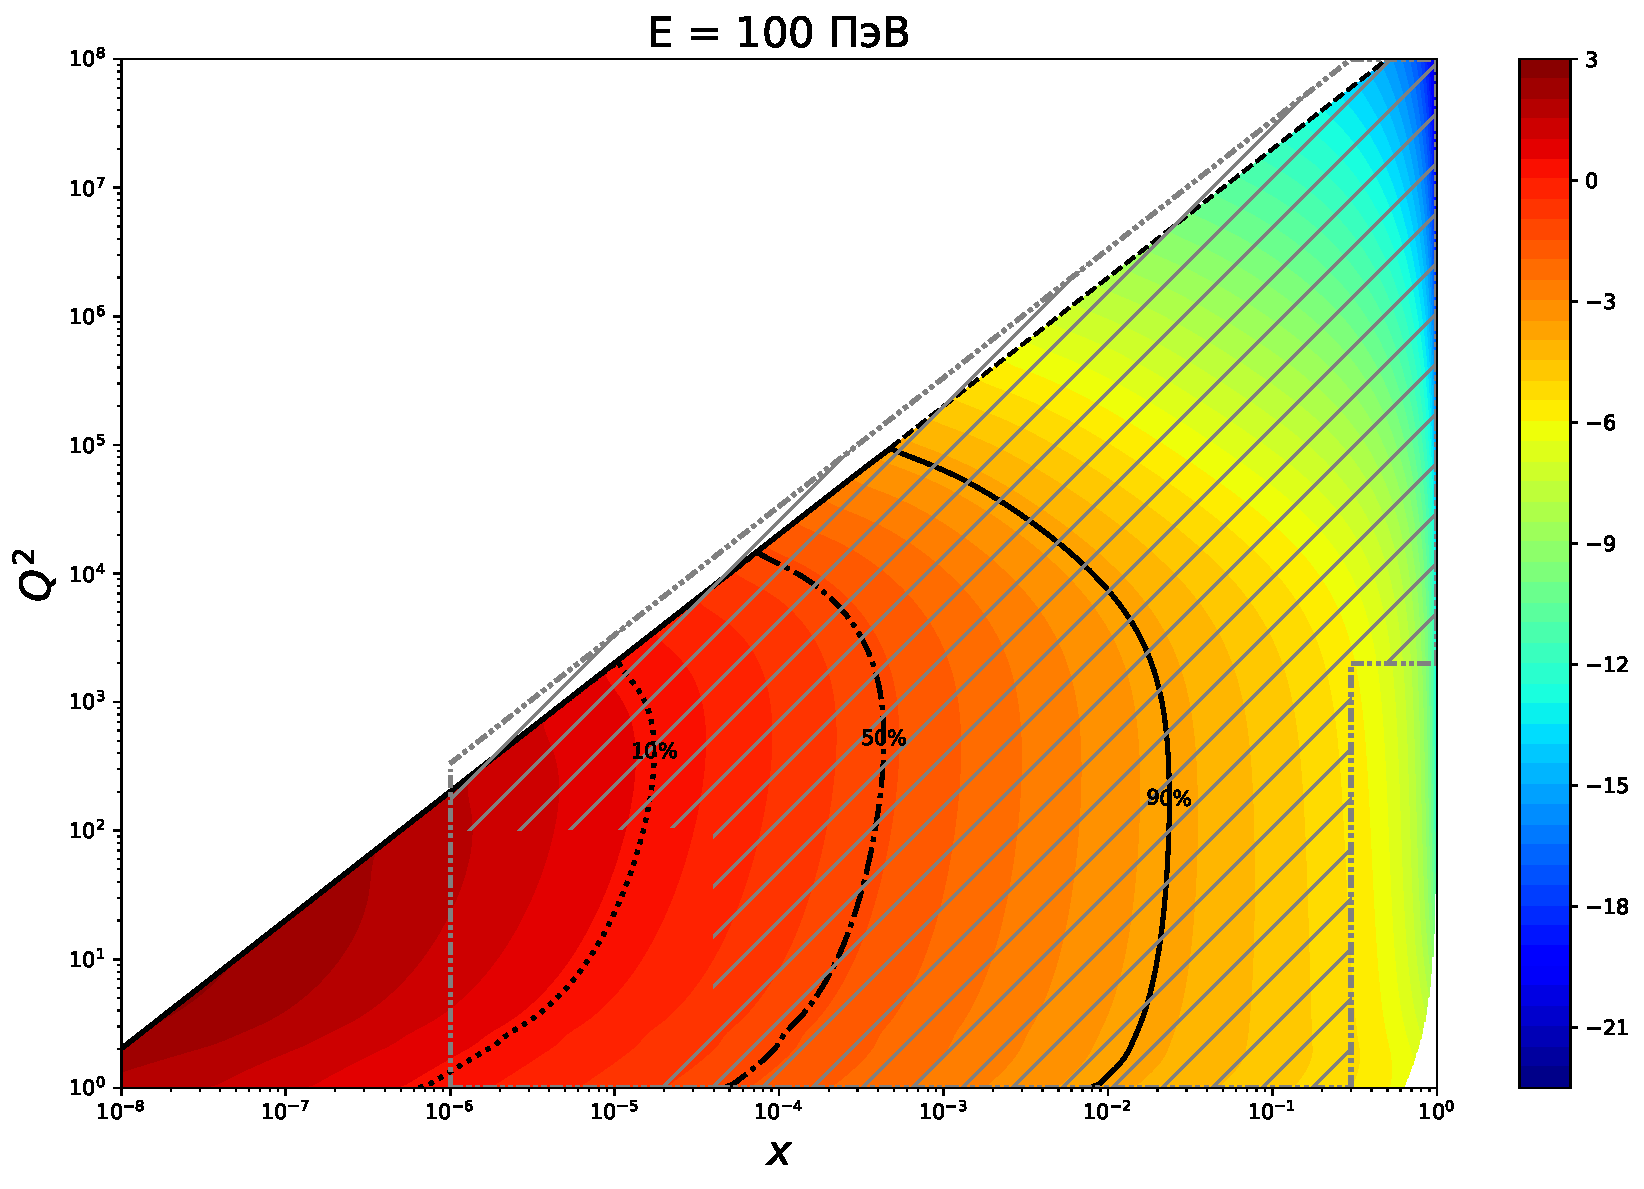
\includegraphics[width=0.8\linewidth]{images/NuProp/cdfxq2_cc_proton_CT18ZNNLO_14_100000000.pdf}
\caption{Дважды дифференциальное ормированное сечение $\frac{1}{\sigma(E_\nu)}\frac{d^2\sigma(E_\nu,x,Q^2)}{dx\,dQ^2}$ как функция $x$ и $Q^2$ для энергии нейтрино $E_{\nu} = 100$ ПэВ. Использованы партонные распределения CTEQ15\cite{ncteq15}.}
\label{fig:diff_xsec_100PeV}
\end{figure}

В области $x\lesssim 10^{-6}$, где экспериметальные данные отсутствуют, $\frac{1}{\sigma(E_\nu)}\frac{d^2\sigma(E_\nu,x,Q^2)}{dx\,dQ^2}$ максимально.  Пунктирные линии в пространстве $x,Q^2$ на рисунках указывают области, где сечения насыщаются до определенного уровня: $10\%$, $50\%$, $90\%$. Можно сделать заключение, что вклад области $x\lesssim 10^{-6}$ порядка $5\%$. В приложении~\ref{sec:examples_extrapolated_region} приведены еще два примера аналогичных распределений для энергий нейтрино 1 ТэВ и 1 ПэВ. 

Более простой способ оценки заключается в том, чтобы пренебречь сложной зависимостью двумерной области $x,Q^2$, в которой существуют экспериментальные измерения, а сосредоточиться только на главной в данном контексте переменной - $x$ Бьёркена. Определим отношение: 
\begin{equation}
\frac{1}{\sigma(E_\nu)}\int\limits_{x}^1\,\frac{d\sigma(E_\nu,x')}{dx'}dx',
\label{eq:CDF_x}
\end{equation}
где 
\[
\frac{d\sigma(E_\nu,x)}{dx} = \int\limits_0^{1}dy\,\frac{d^2\sigma(E_\nu,x,y)}{dx\,dy}.
\]
На рис.~\ref{fig:CDF_x} приведена функция~\eqref{eq:CDF_x} в зависимости от $x$ и $Q^2$ для треё значений энергии нейтрино $E_{\nu}= $ 1 ТэВ, 1 ПэВ, 100 ПэВ.
\begin{figure}[!h]
\centering
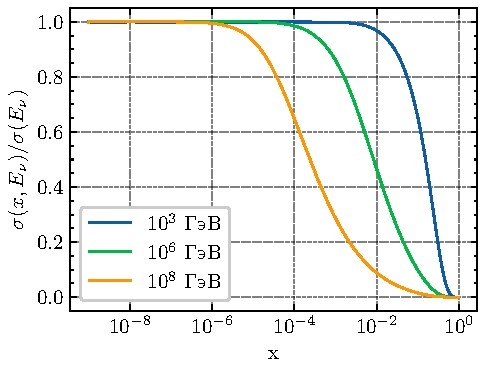
\includegraphics[width=0.8\linewidth]{images/NuProp/cdfxy_plot_CT18ZNNLO_14.pdf}
\caption{Функция $\int\limits_{x}^1\,\frac{1}{\sigma(E_\nu)}\frac{d\sigma(E_\nu,x')}{dx'}dx'$ в зависимости от $x$ и $Q^2$ для треё значений энергии нейтрино $E_{\nu}= $ 1 ТэВ, 1 ПэВ, 100 ПэВ. Использованы партонные распределения CTEQ15\cite{ncteq15}.}
\label{fig:CDF_x}
\end{figure}


\subsection{Полное сечение и его вариация от параметризации}
Из первых принципов довольно сложно оценить вклад неисследованной области в величину полного сечения. Косвенный метод - использовать вариацию в полном сечении при использование различных теоретических параметризаций.  На рис.~\ref{fig:xsec_total} показана зависимость полного сечения взаимодействия мюонного нейтрино на нуклоне от энергии для различных партонных распределений. Также, приведена вариация полного сечения, связанная с использовании разных наборов партонных распределений. Можно сделать вывод о том, что оценка на уровне $5\%$ вариации отвечает наблюдению из предыдущего раздела.

\begin{figure}[!h]
\centering
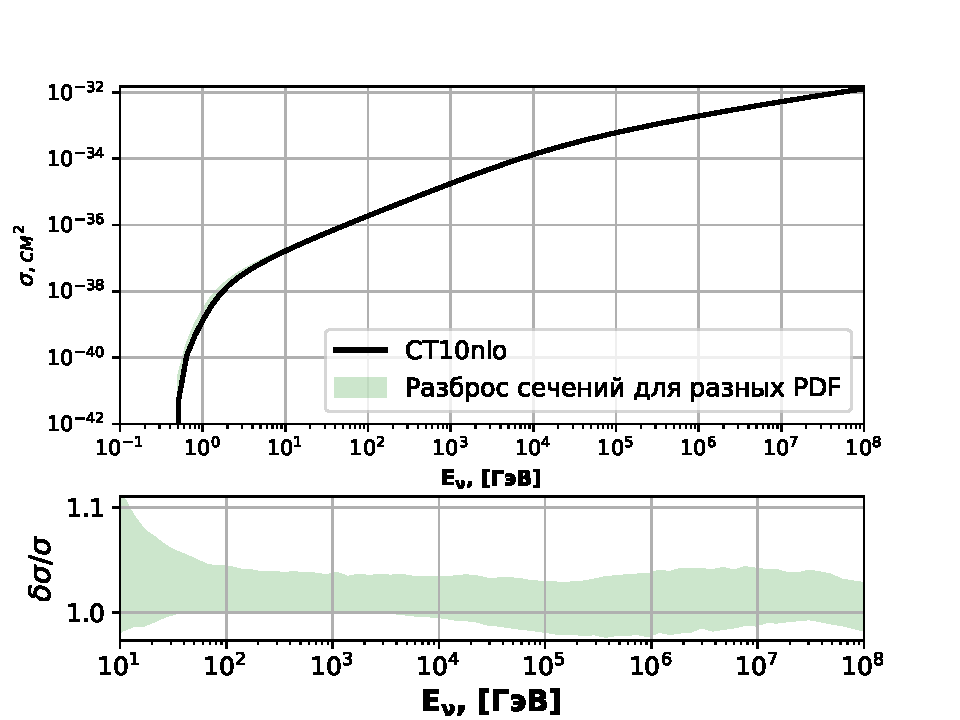
\includegraphics[width=\linewidth]{images/NuProp/xs_vs_enu.pdf}
\caption{Полные сечения взаимодействия мюонного нейтрино на нуклоне в зависимости от энергии $E_\nu$ для партонных распределений \texttt{CT10nlo}. Полоса отвечает вариации полного сечения при использовании других наборов партонных распределений (\texttt{CT18ZNNLO}, \texttt{nCTEQ15}, \texttt{TUJU19\_nlo}).} 
\label{fig:xsec_total}
\end{figure}

\section{Программный пакет \texttt{NuPropagator}}

\subsection{Общее описание и структура}

Пакет \texttt{NuPropagator}~\cite{nupropagator2022} представляет собой модуль для моделирования прохождения потоков нейтрино через вещество, в частности через Землю, с учётом взаимодействий по заряженному и нейтральному токам. Он реализует итеративный метод на основе $\mathcal{Z}$-фактора, что позволяет учитывать регенерацию нейтрино при рассеянии на нуклонах. Пакет написан на языке \texttt{Python3} и поддерживается через платформу \texttt{PyPI}, что обеспечивает его доступность и простоту интеграции в существующие симуляционные цепочки.

\begin{figure}[!h]
\centering
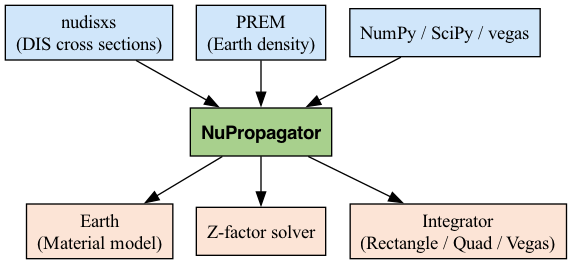
\includegraphics[width=\linewidth]{images/nupropagator_diagram.png}
\caption{Структура программного пакета \texttt{nupropagator} и его зависимости.}
\label{fig:nupropagator1}
\end{figure}

\subsection{Физическая модель}

Пакет \texttt{NuPropagator} использует следующие физические компоненты:
\begin{itemize}
  \item модель плотности Земли (PREM);
  \item сечения взаимодействия нейтрино с нуклонами, предоставляемые пакетом \texttt{nudisxs};
  \item итерационный метод Z-фактора для расчёта эволюции нейтринного спектра.
\end{itemize}

\subsection{Модель плотности Земли и расчёт толщины}

В качестве модели плотности используется Предварительная эталонная модель Земли (PREM)~\cite{dziewonskiPREM1981}, которая предполагает сферическую симметрию и описывает плотность, давление и другие параметры как функции радиуса. Плотность в модели представлена на рис.~\ref{PREM}.

\begin{figure}[!h]
\centering
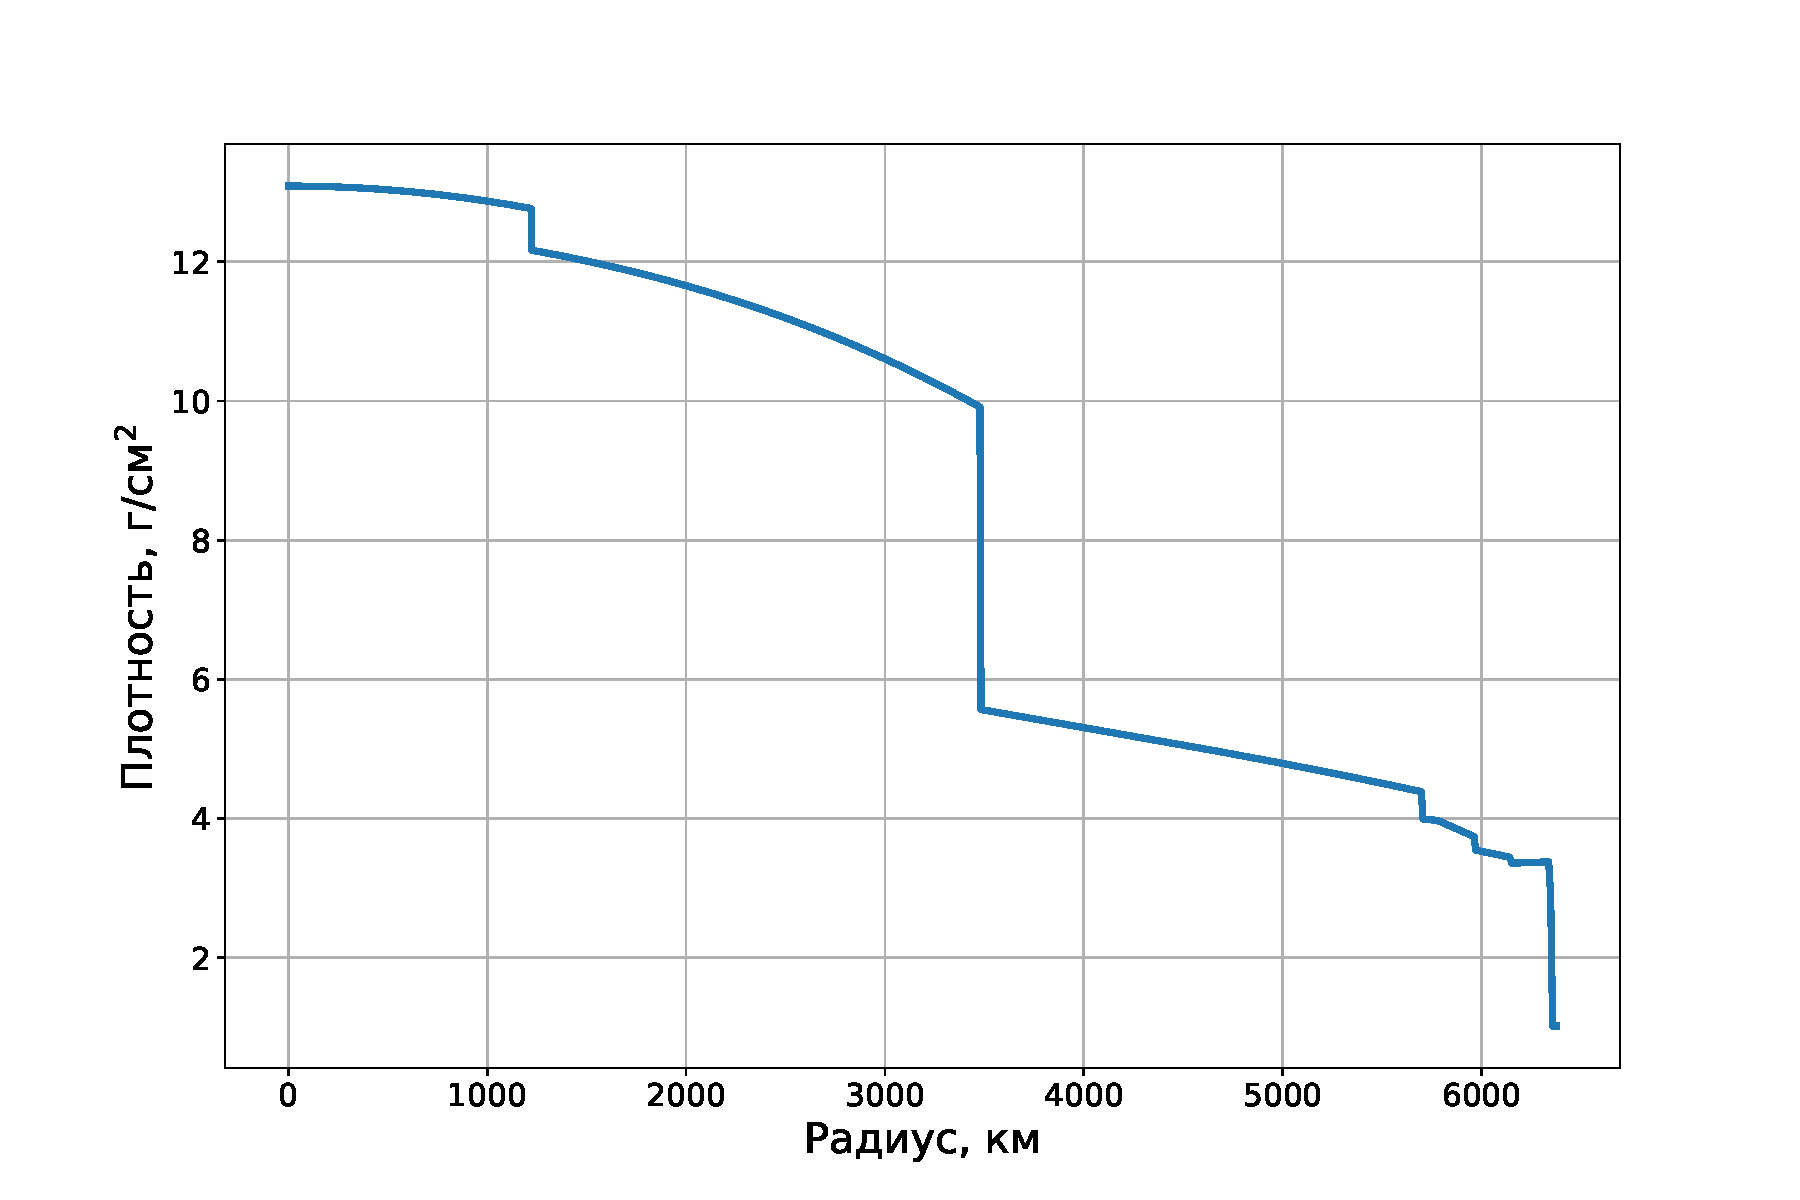
\includegraphics[width=\linewidth]{images/NuProp/PREM.pdf}
\caption{Плотность вещества в модели Земли PREM.}
\label{PREM}
\end{figure}

Расчёт толщины вещества, проходимого нейтрино, осуществляется интегрированием плотности вдоль траектории. Поддерживаются несколько численных методов: метод прямоугольников, квадратурный метод \texttt{quad} из \texttt{SciPy}, и метод Монте-Карло \texttt{vegas}. Изотопный состав вещества задаётся в модуле Earth пакета \texttt{NuPropagator}.

\subsection{Метод Z-фактора}

Z-фактор представляет собой поправку к затуханию потока нейтрино, учитывающую регенерацию за счёт нейтрального тока. Метод подробно описан в работе~\cite{naumov1999} и базируется на решении следующего уравнения переноса нейтрино:
\begin{equation}
\frac{\partial F_{\nu}(x,E)}{\partial x} = \frac{1}{\lambda_{\nu}(E)}\left[ \int\limits_0^1\frac{dy}{1-y}\Phi_{\nu}(y,E) F_{\nu}(x,E_y) - F_{\nu}(x,E) \right],
\end{equation}
где $F_{\nu}(x,E)$ — поток нейтрино после прохождения толщины $x$, $E_y = E/(1-y)$, $\lambda{E}$ - полное сечение взаимодействия нейтрино с веществом, а $\Phi_{\nu}(y,E)$ — распределение по передаче энергии, определяемое следующей формулой:
\begin{equation}
    \Phi_{\nu}(y,E) = \frac{\sum\limits_{T\in \{n,p,e\}}N_T\frac{d\sigma_{\nu T}}{dy}(y,E_y)}{\sum\limits_{T\in \{n,p,e\}}N_T\sigma_{\nu T}(E)}
\end{equation}

Предполагаемое решение имеет вид:
\begin{equation}
F_{\nu}(x,E) = F^{0}_{\nu}(E)\exp\left(-\frac{x}{\Lambda_{\nu}(x,E)}\right),
\end{equation}
где 
\begin{equation}
\Lambda_{\nu}(x,E) = \frac{\lambda_{\nu}(E)}{1 - \mathcal{Z}_{\nu}(x,E)}.
\end{equation}

\subsection{Итерационный метод и его реализация}

Решение уравнения для $\mathcal{Z}_{\nu}(x,E)$ реализуется итерационно, начиная с $\mathcal{Z}^{(0)}$ и строя следующие приближения по схеме:
\begin{equation}
\mathcal{Z}^{(n+1)}_{\nu}(x,E) = \int\limits_0^x dx' \int\limits_0^1 dy\,\eta_{\nu}(y,E)\Phi_{\nu}(y,E)\exp\left[ -x'D^{(n)}_{\nu}(x',E,E_y) \right],
\end{equation}
где $\eta_{\nu}(y,E)$ — весовой фактор, определяемый формой начального спектра. Точное выражение для $\eta_{\nu}(y,E)$ имеет следующий вид: 
\begin{equation}
    \eta_{\nu}(y,E) = \frac{F^0_{\nu}(E_y)}{(1-y)F^0_{\nu}(E)}.
\end{equation}
Выражение для фактора $D^{(n)}_{\nu}(x, E, E_y)$ имеет следующий вид:
\begin{equation}
    D^{(n)}_{\nu}(x, E, E_y) = \frac{1-\mathcal{Z}_{\nu}^{(n)}(x, E_y)}{\lambda(E_y)} - \frac{1-\mathcal{Z}_{\nu}^{(n)}(x, E)}{\lambda(E)}
\end{equation}
Реализация учитывает как исчезновение нейтрино за счёт заряженного тока, так и эффект регенерации от нейтрального тока. Конечная плотность потока описывается экспоненциальным затуханием с учётом эффективной длины пробега:
\begin{equation}
P(E,x) = \exp(-x/\lambda_{\nu}(E)), \quad x = \int\rho(l)\,dl.
\end{equation}
\subsection{Сравнение с другими программными пакетами}
 Проведем сравнение результатов, полученных с помощью двух програмнных пакетов: \texttt{nuFATE}~\cite{Vincent_2017} и \texttt{nupropagator}. Будем сравнивать потоки мюонного нейтрино, приходящих под разными углами после прохождения через землю в некоторой точке, находящейся на глубине 1 км от поверхности Земли. В качестве нейтринного потока на поверхности земли был использован степенной поток $E^{-2}$.
\begin{figure}[!h]
\centering
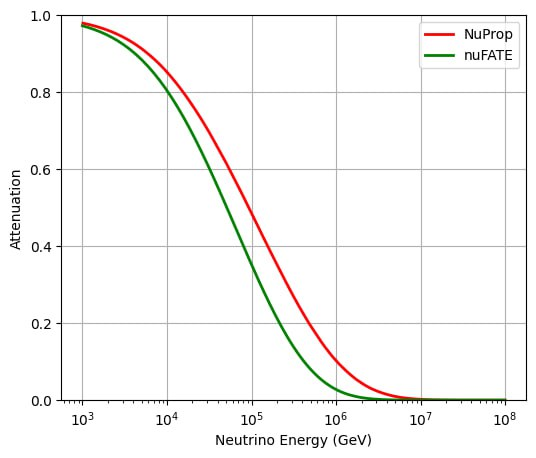
\includegraphics[width=\linewidth]{images/NuProp/compare_fluxes.jpg}
\caption{Сравнение потоков, полученных с помощью \texttt{nuFATE} и \texttt{Nupropagator} для разных углов прилета нейтрино.}
\label{fig:flux_compare}
\end{figure}
Как можно видеть из рис.~\ref{fig:flux_compare} результаты находятся в полном согласии. 



\subsection{Дополнительные возможности}
% (Оставьте место для дополнения при необходимости)

\subsection{Интеграция с другими модулями}
% (Добавьте описание связей с другими компонентами симуляционного фреймворка)

\subsection{Поддержка и установка}

Пакет \texttt{NuPropagator} доступен через \texttt{PyPI} и может быть установлен командой:
\begin{verbatim}
pip install nupropagator
\end{verbatim}
Полная документация доступна на странице проекта, включающей примеры использования и описание API.

\section{Чувствительность к структуре Земли}
%\subsection{Потоки как функция зенитного угла}
%\subsection{Зависимость от энергии}
\subsection{Спектроскопия ядра Земли с нейтрино}
При прохождении нейтрино сквозь Землю мы должны учитывать, что нейтрино в толще земли может взаимодействовать посредством заряженного и нейтрального токов. В качестве примера рассмотрим следующий модельный поток нейтрино на поверхности Земли: 
\begin{equation}
    F_{\nu}^{0}(E) = K\left(\frac{E_0}{E}\right)^{\gamma+1} (1+E_0/E)^{-\alpha}\phi\left(\frac{E}{E_{cut}}\right),
\end{equation}
где $\phi_{cut}(t)$ - некоторая функция, предназначенная для резкого обрезания потоков при энергиях выше некоторого порога. В качестве такой функции возьмем следующую функцию:
\begin{equation}
    \phi(t) = (1+\tan(\pi t/2))^{-1}
\end{equation}
В дальнейшем будем считать, что $\gamma = 1$ и $\alpha = 0.5$.
В качестве точки взаимодействия нейтрино возьмем точку на глубине 1 км от поверхности Земли. Эволюцию потоков нейтрино при прохождении сквозь Землю можно увидеть на рис. (\ref{EF1}). Здесь $\theta_d$ - угол прилета нейтрино относительно детектора (схематическое расположение углов можно увидеть на рис. (\ref{EF1}) справа), $\Phi_{CC}(\theta_d, E)$  - потоки нейтрино в детекторе, если бы мы учитывали изменение только за счет заряженного тока, $\Phi_{CC+NC}(\theta_d, E)$  - потоки нейтрино в детекторе, если бы мы учитывали изменение за счет заряженного и нейтрального токов. Можно видеть, что при энергиях нейтрино выше 1 ПэВ нейтральный ток начинает оказывать большой эффект при распространении нейтрино сквозь Землю. Особенно эффект становится ощутим, если траектория нейтрино проходит через ядро Земли. Данная картинка подсказывает нам эксперимент по спектрографии Земли. Если взять пучок нейтрино высоких энергий (1 ТэВ) и пустить его сквозь Землю по диаметру, поставив два детектора с противоположных сторон, мы сможем измерять потоки нейтрино до и после их прохождения через Землю. Так как при распространении нейтрино практически не изменяет своего направления, можно учесть эффект поглощения нейтрино за счет заряженного тока. Таким образом, превышение потоков нейтрино во втором детекторе от ожидаемых потоков (изменившихся только за счет поглощения) позволит оценить плотность ядра Земли (т. к. основной эффект увеличения потоков дает именно ядро).   
\begin{figure}[!h]
\centering
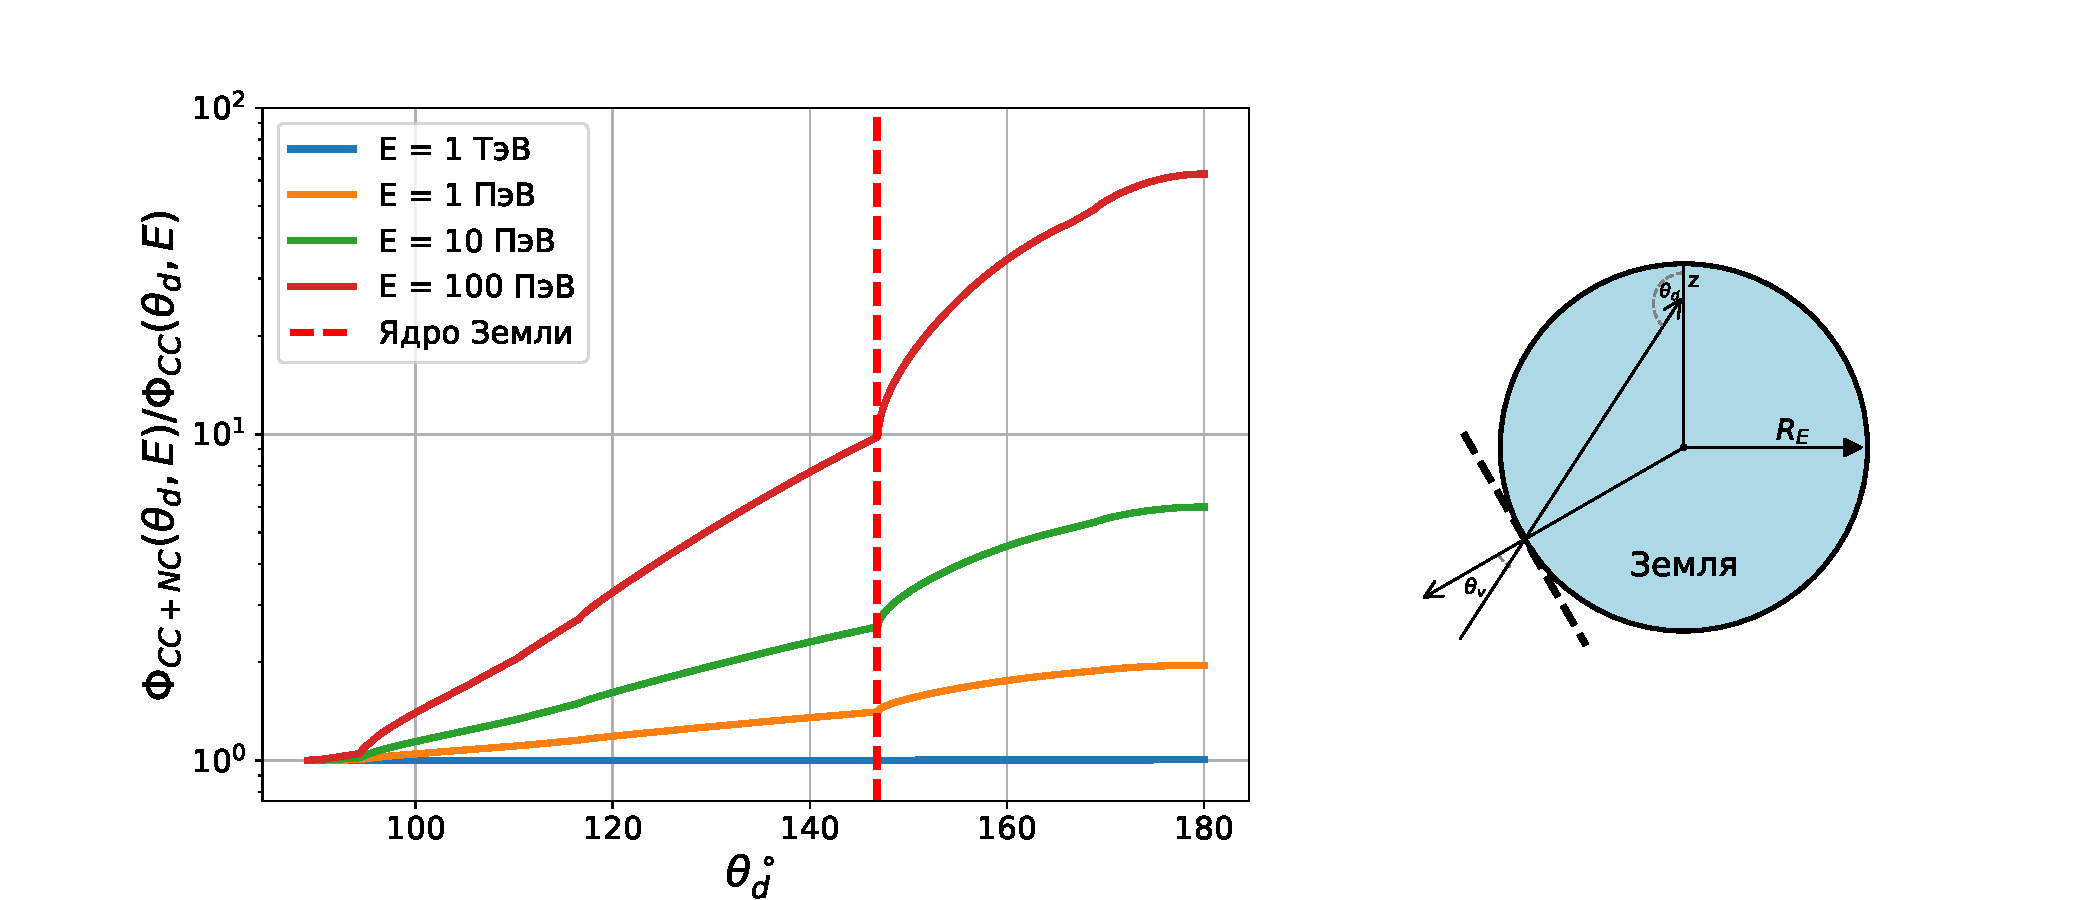
\includegraphics[width=1.1\linewidth]{images/NuProp/rhh12zf_flux_index_CT18ZNNLO.pdf}
\caption{Вклад взаимодействий нейтрино за счет нейтрального тока в общий поток в точке наблюдения потока в зависимости от угла прилета нейтрино отностиельно детектора для разных значений энергии нейтрино. Здесь $z$ - глубина, на которой находится детектор, $\theta_d$ - угол прилета нейтрино, относительно детектора, $\theta_n$ - угол прилета нейтрино, относительно нормали к Земле, $R_E$ - Радиус Земли.}
\label{EF1}
\end{figure}
При распространении нейтрино от одной точки в другую через толщу вещества учитывается как обычный фактор затухания нейтрино, так и фактор, связанный с регенерацией потока (учет реакций, когда конечным лептоном является также нейтрино). В соответствии с процедурой, описанной ранее, для потоков мюонных нейтрино можно построить соответствующую экспоненциальную поправку к затуханию. Полную же картину распространения нейтрино можно увидеть на рис. (\ref{EF2}).
\subsection{Поглощение нейтрино в среде }
 Полную картину распространения нейтрино в зависимости от энергии нейтрино и зенитного угла относительно детектора  можно увидеть на рис. (\ref{EF2}). Здесь учтено поглощение потока, которое дается экспоненциальной поправкой, и регенерация потока, рассчитанная с помощью процедуры $\mathcal{Z}$-фактора.
 \begin{figure}[!h]
\centering
\includegraphics[width=1.1\linewidth]{images/NuProp/rzf_2dxsTUJU19_nlo_2_1.png}
\caption{Вероятность прохождения нейтрино сквозь Землю в зависимости от энергии и зенитного угла, измеряющегося относительно детектора.}
\label{EF2}
\end{figure}
\subsection{Поглощение за счет нейтрального и заряженного токов}
В конце зададимся вопросом, как изменяется показатель потока при прохождении нейтрино сквозь Землю за счёт разных взаимодействий. Предположим, что начальный и конечный потоки имеют форму 
\begin{equation}
    F_{in/fin}(E) = \Phi_0 E^{-\gamma_{in/fin}(E)}.
\end{equation}
На рис. (\ref{EF3}) можно видеть, что показатель потока начинает сильно изменяться при энергиях выше 10 ТэВ. Таким образом, для нейтрино высоких энергий, проходящих сквозь Землю, спектр будет сильно изменяться, поэтому количество событий для таких нейтрино будет сильно меньше ожидаемых. Нейтрино же, летящие сверху, не подвергнутся такому подавлению потока.    
\begin{figure}[!h]
\centering
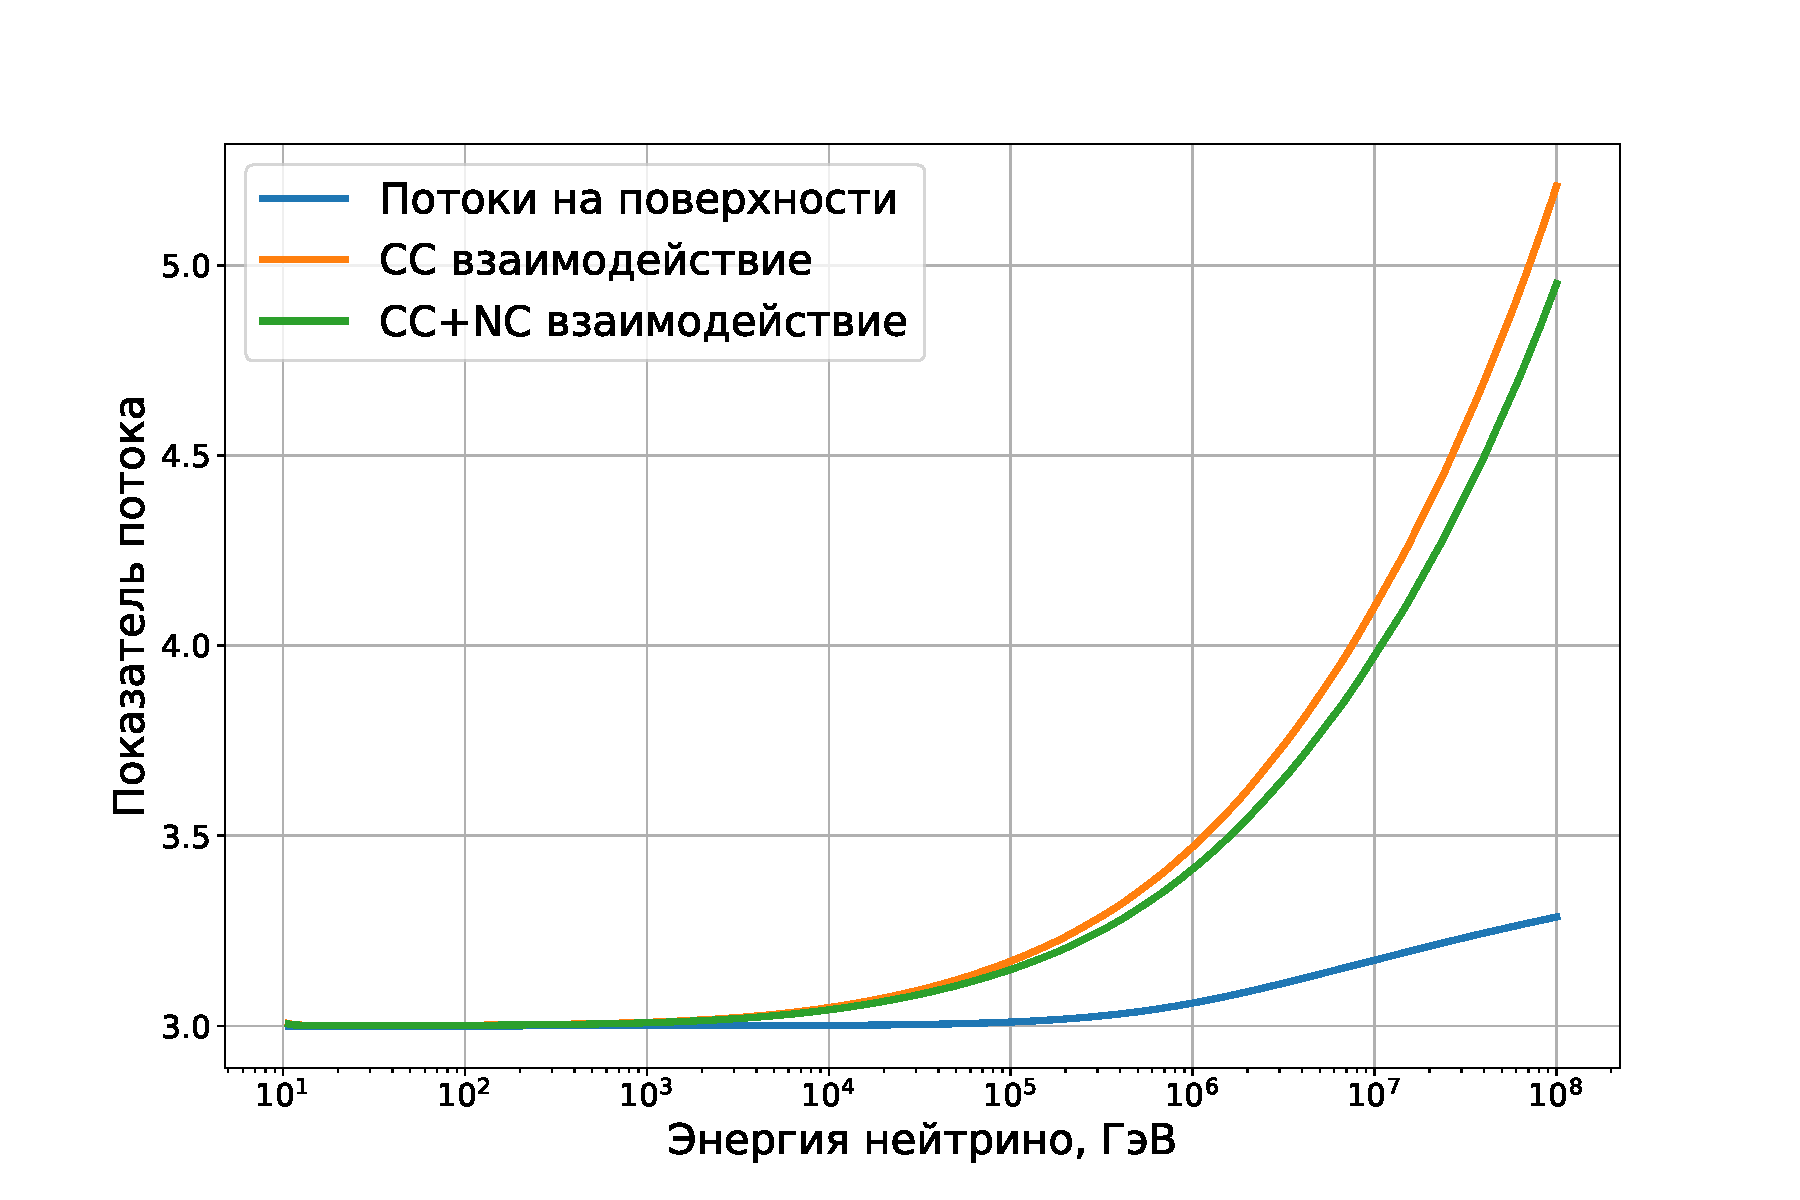
\includegraphics[width=1.1\linewidth]{images/NuProp/rzf_flux_index_CT18ZNNLO.pdf}
\caption{Изменение показателя потока нейтрино для пучка, проходящего сквозь Землю в зависимости от энергии при учете разных типов взаимодействия.}
\label{EF3}
\end{figure}
\subsection{Томография Земли с помощью нейтрино}
Рассмотрим возможность уточнить плотность Земли с помощью нейтрино. На данный момент вся информация о плотности Земли получена косвенным образом из сейсмологических данных~\cite{dziewonskiPREM1981}. Однако, можно получать также информацию о плотности с помощью распространения нейтрино в Земле. Одни анализы основаны на осцилляциях нейтрино низких энергий в веществе. В случае же высоких энергий длина осцилляции намного больше радиуса Земли, поэтому осцилляциями можно пренебречь. Однако есть другой способ, основанный на том, что при прохождении нейтрино сквозь Землю происходят два конкурирующих процесса. С одной стороны, потоки нейтрино убывают за счет поглощения нейтрино в среде. С другой стороны, потоки перераспределяются за счет взаимодействия по нейтральному току (обсуждавшийся выше эффект регенерации). В зависимости от длины пути и от плотности вещества вдоль этого пути, мы будем получать разные числа событий в детекторе.


В данной работе мы проведем анализ, предположив, что у нас есть две гипотезы: $H_0$ и $H_1$. Гипотеза $H_0$ будет утверждением о том, что модель плотности PREM верна. В качестве альтернативной гипотезы будем рассматривать простейшие отклонения от данной модели.   
Рассмотрим три альтернативные модели: модель с усредненным ядром, модель с линейным ядром и модель с усредненными мантией и ядром. Анализ будем проводим с помощью статистики $\chi^2$. Найдем полные числа событий нейтринном телескопе объемом $1\text{ км}^3$ за один год для каждой из гипотез и на основании статистики примем либо отклоним гипотезу $H_0$. $\chi^2$ будем рассчитывать по формуле 
\begin{equation}
    \Delta\chi^2 = 2\sum\limits_{ij}(N_{ij}^{(0)} - N_{ij}^{(1)}+N_{ij}^{(1)}\ln(N_{ij}^{(1)}/N_{ij}^{(0)})),
\end{equation}
где $N^{k}_{ij}$ - количество нейтринных событий в определенном диапазоне по углам и энергии, соответствующих $k$-й гипотезе. 
\begin{enumerate}
    \item \textbf{Усредненное ядро и мантия.} В качестве альтернативной гипотезы возьмем модель плотности, равной $5.51\text{ г/см}^3$ в области внутреннего ядра, внешнего ядра и мантии (до 5600 км).В остальной же области модель будет совпадать с моделью PREM. Для данной пары ($H_0$,$H_1$) получилось $\Delta\chi^2 = 12.2$, что соответствует статистической значимости на уровне $3.5\sigma$.   
    \begin{figure}[!h]
    \centering
    \includegraphics[width=1.1\linewidth]{images/NuProp/chi2_rzf_2dxsCT18ZNNLO_PREM_vs_PREM_man_and_ker.png}
    \caption{Распределение $\Delta\chi^2$, полученное на основе сравнения чисел нейтринных событий в предположении двух гипотез, где в качестве альтернативной гипотезы взята гипотеза усредненного ядра и мантии}
    \label{NuTom1}
    \end{figure}
    \item \textbf{Усредненное ядро.} В качестве альтернативной гипотезы возьмем модель плотности, равной $11.87\text{ г/см}^3$ в области внутреннего ядра и внешнего ядра. В остальной же области модель будет совпадать с моделью PREM. Для данной пары ($H_0$,$H_1$) получилось $\Delta\chi^2 = 0.15$, что соответствует статистической значимости на уровне $0.4\sigma$. Если проводить наблюдения в течение 25 лет или же анализировать данные, полученные с помощью очень больших нейтринных телескопов (объемом $30 \text{ км}^3$, например), то результат станет статистически значимым на уровне $2\sigma$.   
    \begin{figure}[!h]
    \centering
    \includegraphics[width=1.1\linewidth]{images/NuProp/chi2_rzf_2dxsCT18ZNNLO_PREM_vs_PREM_av_ext_ker.png}
    \caption{Распределение $\Delta\chi^2$, полученное на основе сравнения чисел нейтринных событий в предположении двух гипотез, где в качестве альтернативной гипотезы взята гипотеза усредненного ядра}
    \label{NuTom2}
    \end{figure}
    \item \textbf{Линейное ядро.} Теперь в качестве альтернативной гипотезы возьмем модель плотности,  где плотность аппроксимируется линейной функцией в области внутреннего ядра и внешнего ядра. В остальной же области модель будет совпадать с моделью PREM. Для данной пары ($H_0$,$H_1$) получилось $\Delta\chi^2 = 0.76$, что соответствует статистической значимости на уровне $0.9\sigma$. Если проводить наблюдения в течение 10 лет, то результат станет статистически значимым на уровне $2.8\sigma$. 
    \begin{figure}[!h]
    \centering
    \includegraphics[width=1.1\linewidth]{images/NuProp/chi2_rzf_2dxsCT18ZNNLO_PREM_vs_PREM_lin_ker.png}
    \caption{Распределение $\Delta\chi^2$, полученное на основе сравнения чисел нейтринных событий в предположении двух гипотез, где в качестве альтернативной гипотезы взята гипотеза линейного ядра}
    \label{NuTom3}
    \end{figure}
\end{enumerate}
На основе распределений статистики $\Delta\chi^2$ (рис.~\ref{NuTom1} - рис.~\ref{NuTom3}) можно видеть, что диапазон энергии, особенно чувствительный для нейтринной томографии  - $10^2 \text{ГэВ}-10^6 \text{ГэВ}$, причем пик приходится на $10^4 \text{ ГэВ}$. В этой области среда становится непрозрачной для нейтрино и, в свою очередь, потоки еще не слишком маленькие, как при больших энергиях. Максимум же по углу зависит от того, какую альтернативную модель плотности мы рассматриваем (при изменении плотности в слое мантии, максимум по углам будет смещаться влево к меньшим углам). 
\subsection{Кинетические уравнения}
Рассмотрим уравнение переноса нейтрино, учитывая поглощение нейтрино и взаимодействие нейтрино в веществе.
\begin{equation}
    \frac{\partial F(E, x)}{\partial x} = -\sigma_{tot}(E)F(E, x) + \int\limits_{0}^1\frac{dy}{1-y}\frac{d\sigma_{tot}}{dy}(E_y, y)F(E_y, x), 
\end{equation}
где $E_y = E/(1-y)$ - энергия нейтрино до возможного рассеяния. Перепишем его в виде системы уравнений:
\begin{equation}
    \begin{cases}
         \frac{\partial F(E, x)}{\partial x} = -\sigma_{tot}(E)F(E, x) + Z(E, x)F(E, x),\\
          Z(E, x) = \int\limits_{0}^1\frac{dy}{1-y}\frac{d\sigma_{tot}}{dy}(E_y, y)F(E_y, x).
    \end{cases}
\end{equation}
Перепишем первое уравнение в интегральном виде:
\begin{equation}
    \begin{cases}
          F(E, x) = F_0(E)\exp{(-\sigma_{tot}(E)x + \int\limits_{0}^1dx_1Z(E, x_1)}),\\
          Z(E, x) = \int\limits_{0}^1\frac{dy}{1-y}\frac{d\sigma_{tot}}{dy}(E_y, y)F(E_y, x).
    \end{cases}
\end{equation}
\begin{equation}
    \begin{cases}
          F(E, x) = F_0(E)\exp{(-\sigma_{tot}(E)x + \int\limits_{0}^1dx_1Z(E, x_1)}),\\
          Z(E, x) = \int\limits_{0}^1\frac{dy}{1-y}\frac{d\sigma_{tot}}{dy}(E_y, y)F(E_y, x).
    \end{cases}
\end{equation}
Таким образом, мы получаем следующее интегральное уравнение: 
\begin{equation}
          F(E, x) = F_0(E)\exp{\left(-\sigma_{tot}(E)x + \int\limits_{0}^1dx_1 \int\limits_{0}^1\frac{dy}{1-y}\frac{d\sigma_{tot}}{dy}(E_y, y)\frac{F(E_y, x)}{F(E,x)}\right)}.
\end{equation}
Решаем его итерациями: 
\begin{equation}
          F^{(n+1)}(E, x) = F_0(E)\exp{\left(-\sigma_{tot}(E)x + \int\limits_{0}^1dx_1 \int\limits_{0}^1\frac{dy}{1-y}\frac{d\sigma_{tot}}{dy}(E_y, y)\frac{F^{(n)}(E_y, x)}{F^{(n)}(E,x)}\right)}.
\end{equation}
В первом приближении имеем: 
\begin{equation}
          F^{(1)}(E, x) = F_0(E)\exp{\left(-x\left[\sigma_{tot}(E) -\int\limits_{0}^1dy\frac{d\sigma_{tot}}{dy}(E_y, y)\eta(E, y)\right]\right)},
\end{equation}
где 
\begin{equation}
    \eta(E,y) = \frac{F_0(E_y)}{(1-y)F_0(E)}.
\end{equation}

\appendix
\subsubsection{Структурные функции и кинематические формулы}
\label{app:structure_functions}

Для случая неполяризованного лептона ненулевыми оказываются следующие функции $A_i$:
\begin{equation}
    \begin{aligned}
        A_1(x, y, E) &= y(xy + a), \\
        A_2(x, y, E) &= 1 - y - \frac{xyM_N}{2E} - \left( \frac{m_{l}}{2E} \right)^2, \\
        A_3(x, y, E) &= y\left( x\left(1 - \frac{y}{2} \right) - \frac{a}{2} \right), \\
        A_4(x, y, E) &= a(xy + a), \\
        A_5(x, y, E) &= -a,
    \end{aligned}
\end{equation}
где $a = m_l^2/(2M_N E)$, а $m_l$ — масса лептона.

В партонной аппроксимации структурные функции выражаются через функции распределения кварков и антикварков:
\begin{equation}
    \begin{aligned}
        F_1(x) &= \frac{1}{2} \sum\limits_{i} e_i^2 \left[ q_i(x) + \bar{q}_i(x) \right], \\
        F_2(x) &= \sum\limits_{i} e_i^2 x \left[ q_i(x) + \bar{q}_i(x) \right], \\
        F_3(x) &= \sum\limits_{i} e_i^2 \left[ q_i(x) - \bar{q}_i(x) \right],
    \end{aligned}
\end{equation}
где $e_i$ — заряд $i$-го кварка в единицах заряда электрона.

Допустимый диапазон квадрата полной массы адронной системы задаётся интервалом $W^2 \in [W^2_{\text{cut}}, W_+^2]$, где $W_{\text{cut}}$ — нижний кинематический порог, а $W_+ = \sqrt{s} - m_l$. При этом пороговая энергия нейтрино равна
\begin{equation}
    E_\nu^{\text{th}} = \frac{(W_{\text{cut}} + m_l)^2 - M_N^2}{2M_N}.
\end{equation}

Допустимая область для переменной Бьёркена $x$ ограничивается значениями:
\begin{equation}
    x^{-}(W_{\text{cut}}) \le x \le x^{+}(W_{\text{cut}}),
\end{equation}
где
\begin{equation}
    x^{\pm}(W_{\text{cut}}) = \frac{a \pm \sqrt{b}}{2c},
\end{equation}
а параметры $a$, $b$, $c$ выражаются через:
\begin{equation}
    \begin{aligned}
        a(W_{\text{cut}}) &= 1 - \frac{[W_{\text{cut}}^2 - M_N^2 - m_l^2][(W_{\text{cut}}^2 - M_N^2)E_\nu + m_l^2 M_N]}{2M_N^2(W_{\text{cut}}^2 - M_N^2)E_\nu^2}, \\
        b(W_{\text{cut}}) &= \left[ 1 - \frac{(W_{\text{cut}} - m_l)^2 - M_N^2}{2M_N E_\nu} \right] \left[ 1 - \frac{(W_{\text{cut}} + m_l)^2 - M_N^2}{2M_N E_\nu} \right], \\
        c(W_{\text{cut}}) &= 1 + \frac{(W_{\text{cut}}^2 - M_N^2 - m_l^2)^2}{4E_\nu^2(W_{\text{cut}}^2 - M_N^2)}.
    \end{aligned}
\end{equation}

После выбора $x$ переменная $y$ выбирается из диапазона:
\begin{equation}
    y^{\text{min}}(E_\nu, W_{\text{cut}}) \le y \le y^+(E_\nu),
\end{equation}
где
\begin{equation}
    \begin{aligned}
        y^{\text{min}}(E_\nu, W_{\text{cut}}) &= \max\left( y^-(E_\nu), y^{\text{cut}}(E_\nu, W_{\text{cut}}) \right), \\
        y^{\text{cut}}(E_\nu, W_{\text{cut}}) &= \frac{W_{\text{cut}}^2 - M_N^2}{2M_N(1 - x)E_\nu},
    \end{aligned}
\end{equation}
и
\begin{equation}
    y^{\pm} = \left[ 1 - \frac{m_l^2}{2E_\nu^2}\left(1 + \frac{E_\nu}{M_N x} \right) \pm \sqrt{ \left(1 - \frac{m_l^2}{2M_N x E_\nu} \right)^2 - \frac{m_l^2}{E_\nu^2} } \right] \left[ 2 + \frac{M_N x}{E_\nu} \right]^{-1}.
\end{equation}


\bibliographystyle{unsrt}
\bibliography{references}

\end{document}